\documentclass{article}
\usepackage[utf8]{inputenc}
\usepackage[english]{babel}
\usepackage{amsmath,amsfonts,amssymb,amsthm}
\usepackage{mathtools}
\usepackage{fancyhdr}
\usepackage{commath}
\usepackage[sc,osf]{mathpazo}
\usepackage{graphicx}
\usepackage{rotating}
\usepackage{float}
\usepackage{subcaption}
\restylefloat{table}
\usepackage{multicol}
\usepackage[dvipsnames]{xcolor}
\usepackage[colorinlistoftodos]{todonotes}
\usepackage{vmargin}  % Administrar márgenes
\setpapersize{A4} % Definir tamaño del papel
\setmargins{3cm} % Margen izquierdo
{1cm} % Margen superior
{15cm} % Área de impresión horizontal
{23.42cm} % Area de impresión vertical
{15mm} % Encabezado
{7mm} % Espacio entre el encabezado y el texto
{10pt} % Pie de página
{3mm} % Espacio entre el pie de página y el texto

\pagestyle{fancy}
\fancyhf{}
\rhead{

\includegraphics[width=4cm,height=1cm]{cropped-iitpal-at-prutor-logo.png}
}
\lhead{Circles | Class XI | Exemplar Problems}
\rfoot{}
\begin{document}
\section*{Practice Questions}
\paragraph{Q1.}Show that the point (x, y) given by $x=\frac{2at}{1+t^2}$ and $y=\frac{a(1-t^2)}{1+t^2}$ lies on a circle for all real values of t such that $-1 <  t < 1$ where a is any given real numbers.

\begin{flushright}
Page-202
\end{flushright}

\paragraph{Q2.}If the lines $3x - 4y + 4 = 0$ and $6x - 8y - 7 = 0$ are tangents to a circle, then find
the radius of the circle.\\
Hint: Distance between given parallel lines gives the diameter of the circle
\begin{flushright}
Page-202
\end{flushright}

\paragraph{Q3.}Find the equation of a circle which touches both the axes and the line $3x - 4y + 8 = 0$
and lies in the third quadrant.\\
Hint:  Let  a  be  the  radius  of  the  circle,  then  (-  a,  -  a)  will  be  centre  and perpendicular distance from the centre to the given line gives the radius of the
circle.
\begin{flushright}
Page-202
\end{flushright}

\paragraph{Q4.}If the line $y = \sqrt{3}  x + k$ touches the circle $x^2 + y^2 = 16$, then find the value of $k$.\\
Hint: Equate perpendicular distance from the centre of the circle to its radius.
\begin{flushright}
Page-202
\end{flushright}

\clearpage


\section*{Solution and Hints}
\paragraph{S1.}\
Given point is,
\begin{equation*}
    x=\frac{2at}{1+t^2},y=\frac{a(1-t^2)}{1+t^2}
\end{equation*}
Put its coordinates in $x^2+y^2$ to see what it gives,
\begin{align*}
    x^2+y^2&=\left(\frac{2at}{1+t^2}\right)^2+\left(\frac{a(1-t^2)}{1+t^2}\right)^2\\
    &=\frac{4a^2t^2+a^2(1-t^2)^2}{(1+t^2)^2}\\
    &=\frac{a^2(1+t^4+2t^2)}{(1+t^2)^2}\\
    &=\frac{a^2(1+t^2)^2}{(1+t^2)^2}\\
    &=a^2
\end{align*}
Now compare it with center-radius form $(x-h)^2+(y-k)^2=r^2$ and we get,
\begin{align*}
    center=(0,0)\\
    radius=a
\end{align*}
\paragraph{S2.}\
Just by looking at st. line equations we can see that they are || lines. They touch circle on ends of diameter line. So distance bwtween these tangents should give us diameter of the circle. Equate both lines coefficients,
\begin{align*}
    3x-4y+4&=0\\
    3x-4y-3.5&=0
\end{align*}
Recall from st. line chapter that distance bwtween two || lines is,
\begin{equation*}
    dist=\left|\frac{c-d}{\sqrt{a^2+b^2}}\right|
\end{equation*}
Compare given st. lines with $ax+by+c=0$ and $ax+by+d=0$ and we get,
\begin{equation*}
    dist=\left|\frac{4-(-3.5)}{\sqrt{3^2+(-4)^2}}\right|
\end{equation*}
By solving above, distance comes out $=1.5$. Since this is the diameter of the circle. Radius is,
\begin{equation*}
    r=\frac{1.5}{2}=0.75 \text{  units}
\end{equation*}
\paragraph{S3.}\
Since circle touches both axes in 3rd quadrant, its center can be assumed to be (-a,-a).  We need to find \textbf{a}.
\begin{figure}[H]
    \centering
    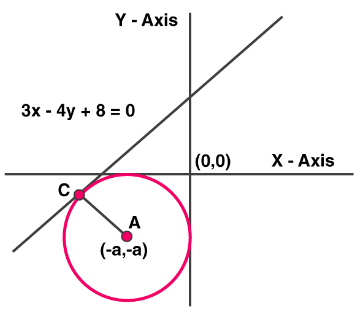
\includegraphics[scale=0.5]{l4_ps1-3.png}
    \caption{Circle in third quadrant}
\end{figure}
Also recall from st. lines chapter that parpendicular distance of st. line($ax+by+c=0$) from a point $(x_1,y_1)$ is given by,
\begin{equation*}
    =\left|\frac{ax_1+by_1+c}{\sqrt{a^2+b^2}}\right|
\end{equation*} 
Since radius(=a) is the distance, we can compare both to get value of a.
\begin{align*}
    a&=\left|\frac{3(-a)-4(-a)+8}{\sqrt{3^2+(-4)^2}}\right|\\
    &=\left|\frac{8+a}{\sqrt{25}}\right|\\
    &=\frac{8+a}{5}\\
    5a&=a+8\\
    a&=2
\end{align*}
Now put values in center radius form of circle,
\begin{equation*}
    (x-(-2))^2+(y-(-2))^2=a^2
\end{equation*}
General form after expanding is,
\begin{equation*}
    x^2+y^2+4x+4y+4=0
\end{equation*}
\paragraph{S4.}\
This problem uses similar concept to Prob-3. We need to compute tangent line's distance from center and equate it with known radius to get value of $k$. Comparing circle equation with center-radius form we get, center $=(0,0)$ and radius $=4$. After converting line equation in $ax+by+c=0$ form and using similar formula as prob-3, 
\begin{equation*}
    \sqrt{3}x-y+k=0
\end{equation*}
Compare distance from formula with radius,
\begin{align*}
    4&=\left|\frac{\sqrt{3}(0)-1(0)+k}{\sqrt{\sqrt{3}^2+(-1)^2}}\right|\\
    4&=\frac{k}{\sqrt{4}}\\
    k&=(4).(2)=8
\end{align*}
Hence the value of $k=8$.
\end{document}